\section{Software Utilizado} \label{pontosSoftware}

Existe uma gama razoável de softwares que são capazes de obter nuvem de pontos a partir de imagens. Dentre eles pode-se citar o Free-D, Insight3D, PhotoModeler e o VisualSFM. Para este trabalho foi utilizado o VisualSFM~\cite{visualSFM} por ser um software gratuito, de fácil uso, correspondência automática das imagens e resultados satisfatórios. As desvantagens dos outros softwares citados são as seguintes:

\begin{itemize}
\item Free-D: A correspondência das imagens é feita manualmente.
\item Insight3d: Ferramenta pouco intuitiva, e de difícil manuseio.
\item PhotoModeler: Ferramenta paga.
\end{itemize}

O VisualSFM recebe como entrada um conjunto de imagens LDR, extrai os pontos de interesse destas imagens e então faz as correspondências entre elas. Uma vez com a correspondência feita, inicializa-se a etapa de recontrução 3D. Nesta etapa são estimados parâmetros da câmera como: distância focal, e distorção radial, além de estimar, para cada imagem, a posição da câmera.

Uma vez com os parâmetros e posições definidas, estima-se as posições dos pontos de interesse que possuem correspondência nas imagens, finalizando a geração da nuvem de pontos. As Figuras \ref{figExemploSFM} mostram um exemplo de geração de nuvem de pontos a partir de imagens LDR.

\begin{figure}[H]
  \centering
  \subfloat[Carrega as imagens LDR.]
  {
    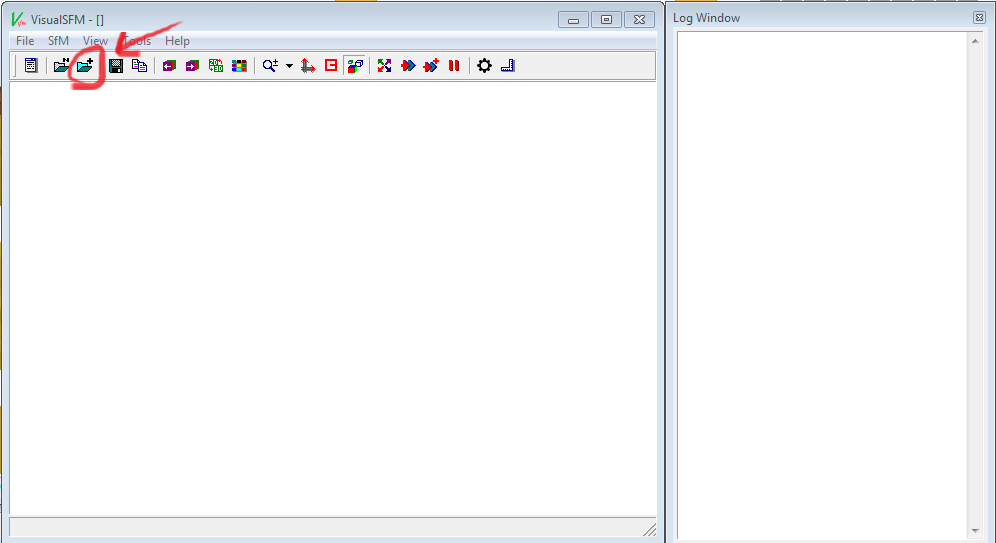
\includegraphics[height=5cm]{exVisualSFM/uso0}
    \label{figExemploSFMA}
  }
  \quad %espaco separador
  \subfloat[Encontra a correspondência entre as imagens.]
  {
    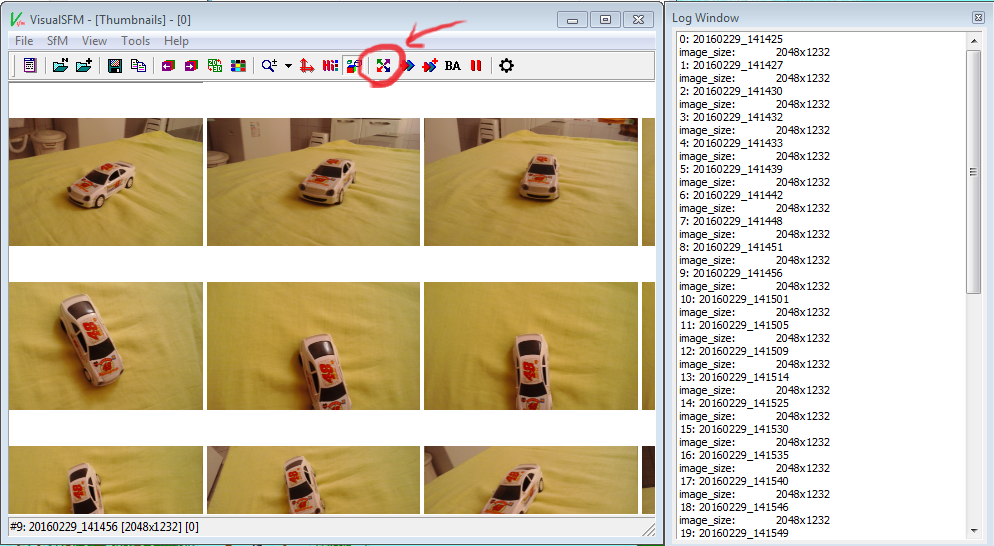
\includegraphics[height=5cm]{exVisualSFM/uso1}
    \label{figExemploSFMB}
  }
  \quad %espaco separador
  \subfloat[Gera a nuvem de pontos.]
  {
    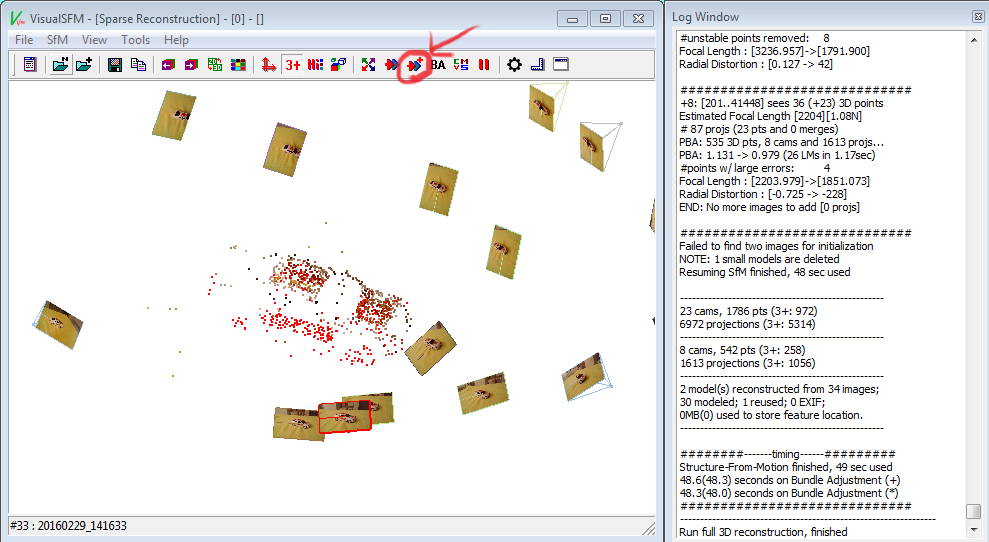
\includegraphics[height=5cm]{exVisualSFM/uso2}
    \label{figExemploSFMC}
  }
  \caption{Exemplo de execução do VisualSFM para a geração de nuvem de pontos a partir de imagens LDR.}
  \label{figExemploSFM}
\end{figure}
